\documentclass[12pt,a4paper]{uebung}

\usepackage[british]{babel}
\usepackage{epsfig}
\usepackage{rotate}
\usepackage{amsmath}
\usepackage{color}
\makeatletter\let\@amsfonts=P\makeatother
\usepackage{graphicx}
\usepackage{typearea}
\usepackage{multicol}
\usepackage{amsfonts}
\usepackage[nounderscore]{syntax}
\usepackage{paralist}
\usepackage{tikz}
\usetikzlibrary{shapes,snakes}
\usepackage{url}
\usepackage{xspace}
%\usepackage{bbm}
\usepackage{listings}
%\usepackage{MnSymbol}
%\usepackage[ruled]{algorithm2e}
\def\NN{{\ensuremath{\mathbbm{N}_0\xspace}}}
\usepackage{fvsw}
\usepackage{tabularx}

\setlength{\textheight}{25cm}

\begin{document}

\newcommand{\Vorlesung}{Formal Methods in Computer Science}
\newcommand{\Semester}{SS 2012}
\newcommand{\Prof}{Univ.~Prof.~Helmut Veith}
\newcommand{\AssisA}{Dr. Igor Konnov}
\newcommand{\AssisB}{Dr. Florian Zuleger}
\newcommand{\AssisC}{Andreas Holzer, M.Sc.}
\newcommand{\AssisD}{Moritz Sinn, M.Sc.}


%\newcommand{\AssisC}{Dipl.-Math. Florian Zuleger}

%\newcommand{\solution}[1]{
%\paragraph{Solution:} #1
%}
\newcommand{\solution}[1]{}

\newcommand\ltlX{\textsf{\textbf{X}}\,}
\newcommand\ltlF{\textsf{\textbf{F}}\,}
\newcommand\ltlG{\textsf{\textbf{G}}\,}
\newcommand\ltlU{\,\textsf{\textbf{U}}\,}
\newcommand\ILTLX[0]{$\mbox{\textsf{ILTL}}_{\mbox{\textsf{-X}}}$}
\newcommand\LTLX[0]{$\mbox{\textsf{LTL}}_{\mbox{\textsf{-X}}}$}

%%%%%%%%%%%%%%%%%%%%%%%%%%%%%%%%%%%%%%%%%%%%%%%%%%%%%%%%%%%%%%%%%%%%%%%%%%%%%%

\Uebungsblatt{4}{Wednesday, 30 May 2012}

%%%%%%%%%%%%%%%%%%%%%%%%%%%%%%%%%%%%%%%%%%%%%%%%%%%%%%%%%%%%%%%%%%%%%%%%%%%%%%

\setlength{\unitlength}{1mm}
{\hfill Version: 3 / 05062012\\}
\begin{tabularx}{\textwidth}{|l|X|}
\hline
\textbf{Name:}& Mustermann \\\hline
\textbf{Vorname:}& Max\\\hline
\textbf{Matr.-nr.:}& 0123456 \\\hline
\textbf{Gruppe:}& Harald Glanzer (0727156), Bernd-Peter Ivanschitz (06XXXX), Lukas Petermann (07XXXX)  \\\hline
\end{tabularx}


%%%%%%%%%%%%%%%%%%%%%%%%%%%%%%%%%%%%%%%%%%%%%%%%%%%%%%%%%%%%%%%%%%%%%%
%% Aufgabe

\begin{center}
\textbf{The deadline for handing in the solution is Sunday, 17th of June, before midnight.}
\end{center}

\Aufgabe[ACTL \& LTL\hfill\textbf{(2 Points)}]
\newcommand{\ACTL}{\mathbf{ACTL}}
\newcommand{\LTL}{\mathbf{LTL}}
\newcommand{\CTLstar}{\mathbf{CTL}^*}
\newcommand{\AP}{\mathbf{AP}}
\newcommand{\true}{\mathbf{true}}
\newcommand{\false}{\mathbf{false}}
\newcommand{\trans}{\mathsf{trans}}
\newcommand{\ltlA}{\textsf{\textbf{A}}\,}
Given an LTL formula $\varphi$ in Negation Normal Form, the following function 
$\mathsf{trans} : \LTL \rightarrow \ACTL$ translates $\varphi$ into an ACTL 
formula $\trans(\varphi)$ as follows:
\begin{center}
\begin{tabular}{l|l}
	$\varphi$ & $\trans(\varphi)$\\
	\hline
	$\true$ & $\true$\\
	$\false$ & $\false$\\
	$a$ & $a$\\
	$\neg a$ & $\neg a$\\
	$\varphi_1 \vee \varphi_2$ & $\trans(\varphi_1) \vee \trans(\varphi_2)$\\
	$\varphi_1 \wedge \varphi_2$ & $\trans(\varphi_1) \wedge \trans(\varphi_1)$\\
	$\mathbf{X} \varphi_1$ & $\mathbf{AX}~\trans(\varphi_1)$\\
	$\mathbf{F} \varphi_1$ & $\mathbf{AF}~\trans(\varphi_1)$\\
	$\mathbf{G} \varphi_1$ & $\mathbf{AG}~\trans(\varphi_1)$\\
	$\varphi_1 \mathbf{U} \varphi_2$ & $\mathbf{A}\left[ \trans(\varphi_1)\;\mathbf{U}\;\trans(\varphi_2) \right]$\\
	$\varphi_1 \mathbf{R} \varphi_2$ & $\mathbf{A}\left[ \trans(\varphi_1)\;\mathbf{R}\;\trans(\varphi_2) \right]$\\
\end{tabular}
\end{center}
The semantics of the ``release'' operator $\mathbf{R}$ is defined as follows:
$$M, \pi \models \varphi_1 \mathbf{R} \varphi_2 \stackrel{def}{\Leftrightarrow} \forall j \geq 0. \pi^j \models \varphi_2 \textnormal{ or } \exists i \geq 0. (\pi^i \models \varphi_1) \wedge (\forall k \leq i. \pi^k \models \varphi_2)$$

\paragraph{a)} Show that, for all $\LTL$ formulas $\varphi$ in negation normal form, the $\CTLstar$ 
formula $\trans(\varphi) \Rightarrow \mathbf{A}\varphi$ is a tautology.
\emph{Hint: Show this by showing that $M, s \models \trans(\varphi)$ implies 
$M, s \models \mathbf{A}\varphi$ for all $\LTL$ formulas $\varphi$ in negation normal form, all Kripke 
structures $M$ and all states $s$ in $M$.
Use induction over the structure of~$\varphi$.}\hfill\textbf{(1 Point)}
 
\begin{tabular}{l l l}
\hline
\hline
(1) & & \\
$M,s\models trans(true)$ & $ \Rightarrow $ & $ M,s\models A\ true$ \\
$M,s\models true $ & $ \Rightarrow $ & $ M,s\models A\ true$ \\
 & $\Rightarrow$ & iff for every path $\pi$ starting from s: $M,\pi \models\ true$ \\
 & & iff s is first state of $\pi$ and $M,s\models true$ \\
\hline
\hline
(2) & & \\
$M,s\models trans(false)$ & $ \Rightarrow $ & $ M,s\models A\ false$ \\
$M,s\models false $ & $ \Rightarrow $ & $ M,s\models A\ false$ \\
$M,s\not\models true$ & $\Rightarrow$ & iff for every path $\pi$ starting from s: $M,\pi \not\models\ true$ \\
 & & iff s is first state of $\pi$ and $M,s\not\models true$ \\
\hline
\hline
(3) & & \\
$M,s\models trans(a)$ & $ \Rightarrow $ & $ M,s\models A\ a$ \\
$M,s\models a $ & $ \Rightarrow $ & $ M,s\models A\ a$ \\
$M,s\models a$ & $\Rightarrow$ & iff for every path $\pi$ starting from s: $M,\pi \models\ a$ \\
 & & iff s is first state of $\pi$ and $M,s\models a$ \\
\hline
\hline
% NOT a
(4) & & \\
$M,s\models trans(\neg a)$ & $ \Rightarrow $ & $ M,s\models A\neg a$ \\
$M,s\models \neg a $ & $ \Rightarrow $ & $ M,s\models A\neg a$ \\
$M,s\not\models a$ & $\Rightarrow$ & $M,s\not\models A\ \ a$ \\
& & iff for every path $\pi$ starting from s: $M,\pi \not\models\ a$ \\
 & & iff s is first state of $\pi$ and $M,s\not\models a$ \\
\end{tabular}
\\
% \begin{tabular}{l l l}
% \hline
% \hline
% % OR operator
% (5) OR & & \\
% $M,s\models trans(\varphi_1 \vee\varphi_2)$ & $ \Rightarrow $ & $ M,s\models A(\varphi_1 \vee \varphi_2)$ \\
% \hline
% $M,s\models trans(\varphi_1) \vee trans(\varphi_2)$ & $ \Rightarrow $ & $ M,s\models A(\varphi_1 \vee \varphi_2)$ \\
% $M,s\models trans(\varphi_1)\ OR\ M,s\models trans(\varphi_2)$ & $ \Rightarrow $ & $ M,s\models A(\varphi_1 \vee \varphi_2)$ \\
% $M,s\models trans(true)\ OR\ M,s\models trans(true)$ & $ \Rightarrow $ & $ M,s\models A(true\vee true)$ \\
% $M,s\models trans(true)$ & $ \Rightarrow $ & $ M,s\models A(true)$ \\
% ... see (1) & & \\
% \hline
% $M,s\models trans(\varphi_1) \vee trans(\varphi_2)$ & $ \Rightarrow $ & $ M,s\models A(\varphi_1 \vee \varphi_2)$ \\
% $M,s\models trans(\varphi_1)\ OR\ M,s\models trans(\varphi_2)$ & $ \Rightarrow $ & $ M,s\models A(\varphi_1 \vee \varphi_2)$ \\
% $M,s\models trans(true)\ OR\ M,s\models trans(false)$ & $ \Rightarrow $ & $ M,s\models A(true\vee false)$ \\
% $M,s\models trans(true)$ & $ \Rightarrow $ & $ M,s\models A(true)$ \\
% ... see (1) & & \\
% \hline
% $M,s\models trans(\varphi_1) \vee trans(\varphi_2)$ & $ \Rightarrow $ & $ M,s\models A(\varphi_1 \vee \varphi_2)$ \\
% $M,s\models trans(\varphi_1)\ OR\ M,s\models trans(\varphi_2)$ & $ \Rightarrow $ & $ M,s\models A(\varphi_1 \vee \varphi_2)$ \\
% $M,s\models trans(false)\ OR\ M,s\models trans(true)$ & $ \Rightarrow $ & $ M,s\models A(false\vee true)$ \\
% $M,s\models trans(true)$ & $ \Rightarrow $ & $ M,s\models A(true)$ \\
% ... see (1) & & \\
% \hline
% $M,s\models trans(\varphi_1) \vee trans(\varphi_2)$ & $ \Rightarrow $ & $ M,s\models A(\varphi_1 \vee \varphi_2)$ \\
% $M,s\models trans(\varphi_1)\ OR\ M,s\models trans(\varphi_2)$ & $ \Rightarrow $ & $ M,s\models A(\varphi_1 \vee \varphi_2)$ \\
% $M,s\models trans(false)\ OR\ M,s\models trans(false)$ & $ \Rightarrow $ & $ M,s\models A(false\vee false)$ \\
% $M,s\models trans(false)$ & $ \Rightarrow $ & $ M,s\models A(false)$ \\
% ... see (2) & & \\
% \hline \\
% $M,s\models trans(\varphi_1) \vee trans(\varphi_2)$ & $ \Rightarrow $ & $ M,s\models A(\varphi_1 \vee \varphi_2)$ \\
% $M,s\models trans(\varphi_1)\ OR\ M,s\models trans(\varphi_2)$ & $ \Rightarrow $ & $ M,s\models A(\varphi_1 \vee \varphi_2)$ \\
% $M,s\models trans(a)\ OR\ M,s\models trans(a)$ & $ \Rightarrow $ & $ M,s\models A(a\vee a)$ \\
% $M,s\models trans(a)$ & $ \Rightarrow $ & $ M,s\models A(a)$ \\
% ... see (3) & & \\
% \end{tabular}
% \\
% \begin{tabular}{l l l}
% \hline \\
% $M,s\models trans(\varphi_1) \vee trans(\varphi_2)$ & $ \Rightarrow $ & $ M,s\models A(\varphi_1 \vee \varphi_2)$ \\
% $M,s\models trans(\varphi_1)\ OR\ M,s\models trans(\varphi_2)$ & $ \Rightarrow $ & $ M,s\models A(\varphi_1 \vee \varphi_2)$ \\
% $M,s\models trans(a)\ OR\ M,s\models trans(\neg a)$ & $ \Rightarrow $ & $ M,s\models A(a\vee\neg a)$ \\
% $M,s\models trans(a)$ & $ \Rightarrow $ & $ M,s\models A(a)$ \\
% ... see (3) & & \\
% \hline \\
% $M,s\models trans(\varphi_1) \vee trans(\varphi_2)$ & $ \Rightarrow $ & $ M,s\models A(\varphi_1 \vee \varphi_2)$ \\
% $M,s\models trans(\varphi_1)\ OR\ M,s\models trans(\varphi_2)$ & $ \Rightarrow $ & $ M,s\models A(\varphi_1 \vee \varphi_2)$ \\
% $M,s\models trans(\neg a)\ OR\ M,s\models trans(a)$ & $ \Rightarrow $ & $ M,s\models A(\neg a\vee a)$ \\
% $M,s\models trans(a)$ & $ \Rightarrow $ & $ M,s\models A(a)$ \\
% ... see (3) & & \\
% 
% \hline \\
% $M,s\models trans(\varphi_1) \vee trans(\varphi_2)$ & $ \Rightarrow $ & $ M,s\models A(\varphi_1 \vee \varphi_2)$ \\
% $M,s\models trans(\varphi_1)\ OR\ M,s\models trans(\varphi_2)$ & $ \Rightarrow $ & $ M,s\models A(\varphi_1 \vee \varphi_2)$ \\
% $M,s\models trans(\neg a)\ OR\ M,s\models trans(\neg a)$ & $ \Rightarrow $ & $ M,s\models A(\neg a\vee\neg a)$ \\
% $M,s\models trans(\neg a)$ & $ \Rightarrow $ & $ M,s\models A\neg a$ \\
% ... see (4) & & \\
%  \hline \\
% $M,s\models trans(\varphi_1) \vee trans(\varphi_2)$ & $ \Rightarrow $ & $ M,s\models A(\varphi_1 \vee \varphi_2)$ \\
% $M,s\models trans(\varphi_1)\ OR\ M,s\models trans(\varphi_2)$ & $ \Rightarrow $ & $ M,s\models A(\varphi_1 \vee \varphi_2)$ \\
% $M,s\models trans(a)\ OR\ M,s\models trans(true)$ & $ \Rightarrow $ & $ M,s\models A(a\vee\ true)$ \\
% $M,s\models trans(true)$ & $ \Rightarrow $ & $ M,s\models A\ true$ \\
% ... see (1) & & \\
%  \hline \\
% $M,s\models trans(\varphi_1) \vee trans(\varphi_2)$ & $ \Rightarrow $ & $ M,s\models A(\varphi_1 \vee \varphi_2)$ \\
% $M,s\models trans(\varphi_1)\ OR\ M,s\models trans(\varphi_2)$ & $ \Rightarrow $ & $ M,s\models A(\varphi_1 \vee \varphi_2)$ \\
% $M,s\models trans(true)\ OR\ M,s\models trans(a)$ & $ \Rightarrow $ & $ M,s\models A(true\vee\ a)$ \\
% $M,s\models trans(true)$ & $ \Rightarrow $ & $ M,s\models A\ true$ \\
% $M,s\models true$ & $ \Rightarrow $ & $ M,s\models A\ true$ \\
% ... see (1) & & \\
%  \hline \\
% $M,s\models trans(\varphi_1) \vee trans(\varphi_2)$ & $ \Rightarrow $ & $ M,s\models A(\varphi_1 \vee \varphi_2)$ \\
% $M,s\models trans(\varphi_1)\ OR\ M,s\models trans(\varphi_2)$ & $ \Rightarrow $ & $ M,s\models A(\varphi_1 \vee \varphi_2)$ \\
% $M,s\models trans(a)\ OR\ M,s\models trans(false)$ & $ \Rightarrow $ & $ M,s\models A(a\vee\ false)$ \\
% $M,s\models trans(a)$ & $ \Rightarrow $ & $ M,s\models A\ a$ \\
% $M,s\models a$ & $ \Rightarrow $ & $ M,s\models A\ a$ \\
% ... see (3) & & \\
%  \hline \\
% $M,s\models trans(\varphi_1) \vee trans(\varphi_2)$ & $ \Rightarrow $ & $ M,s\models A(\varphi_1 \vee \varphi_2)$ \\
% $M,s\models trans(\varphi_1)\ OR\ M,s\models trans(\varphi_2)$ & $ \Rightarrow $ & $ M,s\models A(\varphi_1 \vee \varphi_2)$ \\
% $M,s\models trans(false)\ OR\ M,s\models trans(a)$ & $ \Rightarrow $ & $ M,s\models A(false\vee\ a)$ \\
% $M,s\models trans(a)$ & $ \Rightarrow $ & $ M,s\models A\ a$ \\
% $M,s\models a$ & $ \Rightarrow $ & $ M,s\models A\ a$ \\
% ... see (3) & & \\
% 
% % NOT a v true
% \hline \\
% $M,s\models trans(\varphi_1) \vee trans(\varphi_2)$ & $ \Rightarrow $ & $ M,s\models A(\varphi_1 \vee \varphi_2)$ \\
% $M,s\models trans(\varphi_1)\ OR\ M,s\models trans(\varphi_2)$ & $ \Rightarrow $ & $ M,s\models A(\varphi_1 \vee \varphi_2)$ \\
% $M,s\models trans(\neg a)\ OR\ M,s\models trans(true)$ & $ \Rightarrow $ & $ M,s\models A(\neg a\vee\ true)$ \\
% $M,s\models trans(true)$ & $ \Rightarrow $ & $ M,s\models A\ a$ \\
% $M,s\models true$ & $ \Rightarrow $ & $ M,s\models A\ true$ \\
% ... see (1) & & \\
% \end{tabular}
% \\
% \begin{tabular}{l l l}
% \hline \\
% $M,s\models trans(\varphi_1) \vee trans(\varphi_2)$ & $ \Rightarrow $ & $ M,s\models A(\varphi_1 \vee \varphi_2)$ \\
% $M,s\models trans(\varphi_1)\ OR\ M,s\models trans(\varphi_2)$ & $ \Rightarrow $ & $ M,s\models A(\varphi_1 \vee \varphi_2)$ \\
% $M,s\models trans(true)\ OR\ M,s\models trans(\neg a)$ & $ \Rightarrow $ & $ M,s\models A(true\vee\ \neg a)$ \\
% $M,s\models trans(true)$ & $ \Rightarrow $ & $ M,s\models A\ true$ \\
% $M,s\models true$ & $ \Rightarrow $ & $ M,s\models A\ true$ \\
% ... see (1) & & \\
% % NOT a v FALSE
% \hline \\
% $M,s\models trans(\varphi_1) \vee trans(\varphi_2)$ & $ \Rightarrow $ & $ M,s\models A(\varphi_1 \vee \varphi_2)$ \\
% $M,s\models trans(\varphi_1)\ OR\ M,s\models trans(\varphi_2)$ & $ \Rightarrow $ & $ M,s\models A(\varphi_1 \vee \varphi_2)$ \\
% $M,s\models trans(\neg a)\ OR\ M,s\models trans(false)$ & $ \Rightarrow $ & $ M,s\models A(\neg a\vee\ false)$ \\
% $M,s\models trans(\neg a)$ & $ \Rightarrow $ & $ M,s\models A\neg a$ \\
% $M,s\models \neg a$ & $ \Rightarrow $ & $ M,s\models A\neg a$ \\
% ... see (2) & & \\
% \hline \\
% $M,s\models trans(\varphi_1) \vee trans(\varphi_2)$ & $ \Rightarrow $ & $ M,s\models A(\varphi_1 \vee \varphi_2)$ \\
% $M,s\models trans(\varphi_1)\ OR\ M,s\models trans(\varphi_2)$ & $ \Rightarrow $ & $ M,s\models A(\varphi_1 \vee \varphi_2)$ \\
% $M,s\models trans(\neg a)\ OR\ M,s\models trans(false)$ & $ \Rightarrow $ & $ M,s\models A(\neg a\vee\ false)$ \\
% $M,s\models trans(\neg)$ & $ \Rightarrow $ & $ M,s\models A\neg a$ \\
% $M,s\models \neg a$ & $ \Rightarrow $ & $ M,s\models A\neg a$ \\
% ... see (2) & & \\
% \end{tabular}
% 
% % AND - operator
% \begin{tabular}{l l l}
%  \hline \\
%  \hline \\
% (5) AND & & \\
% analouge to (4), the distributivity of $\wedge$ holds here too,\\
% so this cases are not shown any more \\
% $M,s\models trans(\varphi_1 \wedge\varphi_2)$ & $ \Rightarrow $ & $ M,s\models A(\varphi_1 \wedge \varphi_2)$ \\
% \hline
% $M,s\models trans(\varphi_1) \wedge trans(\varphi_2)$ & $ \Rightarrow $ & $ M,s\models A(\varphi_1 \wedge \varphi_2)$ \\
% $M,s\models trans(\varphi_1)\ AND\ M,s\models trans(\varphi_2)$ & $ \Rightarrow $ & $ M,s\models A(\varphi_1 \wedge \varphi_2)$ \\
% $M,s\models trans(true)\ AND\ M,s\models trans(true)$ & $ \Rightarrow $ & $ M,s\models A(true\wedge true)$ \\
% $M,s\models trans(true)$ & $ \Rightarrow $ & $ M,s\models A(true)$ \\
% ... see (1) & & \\
% \hline
% $M,s\models trans(\varphi_1) \wedge trans(\varphi_2)$ & $ \Rightarrow $ & $ M,s\models A(\varphi_1 \wedge \varphi_2)$ \\
% $M,s\models trans(\varphi_1)\ OR\ M,s\models trans(\varphi_2)$ & $ \Rightarrow $ & $ M,s\models A(\varphi_1 \vee \varphi_2)$ \\
% $M,s\models trans(true)\ AND\ M,s\models trans(false)$ & $ \Rightarrow $ & $ M,s\models A(true \wedge false)$ \\
% $M,s\models trans(false)$ & $ \Rightarrow $ & $ M,s\models A(false)$ \\
% ... see (2) & & \\
% \hline
% $M,s\models trans(\varphi_1) \wedge trans(\varphi_2)$ & $ \Rightarrow $ & $ M,s\models A(\varphi_1 \wedge \varphi_2)$ \\
% $M,s\models trans(\varphi_1)\ OR\ M,s\models trans(\varphi_2)$ & $ \Rightarrow $ & $ M,s\models A(\varphi_1 \vee \varphi_2)$ \\
% $M,s\models trans(false)\ OR\ M,s\models trans(false)$ & $ \Rightarrow $ & $ M,s\models A(false\vee false)$ \\
% $M,s\models trans(false)$ & $ \Rightarrow $ & $ M,s\models A(false)$ \\
% ... see (2) & & \\
% \hline
% $M,s\models trans(\varphi_1) \wedge trans(\varphi_2)$ & $ \Rightarrow $ & $ M,s\models A(\varphi_1 \wedge \varphi_2)$ \\
% $M,s\models trans(\varphi_1)\ OR\ M,s\models trans(\varphi_2)$ & $ \Rightarrow $ & $ M,s\models A(\varphi_1 \vee \varphi_2)$ \\
% $M,s\models trans(a)\ OR\ M,s\models trans(a)$ & $ \Rightarrow $ & $ M,s\models A(a\vee a)$ \\
% $M,s\models trans(a)$ & $ \Rightarrow $ & $ M,s\models A(a)$ \\
% ... see (3) & & \\
% \end{tabular}


% X - operator
\begin{tabular}{l l l}
 \hline \\
 \hline \\

$M,s\models AX\ trans(\varphi)$ & $ \Rightarrow $ & $ M,s\models AX \varphi$ \\
$ \Leftrightarrow \forall$ paths starting at $s_0.M, \pi \models X\trans(\varphi)$ & &  $\Leftrightarrow \forall$ paths starting at $s_0.M, \pi \models X(\varphi)$ \\
$ \Leftrightarrow \forall$ paths starting at $s_0.M, \pi^1 \models \trans(\varphi)$ & & $ \Leftrightarrow \forall$ paths starting at $s_0.M, \pi^1 \models \varphi$\\
$ \Leftrightarrow \forall$ paths starting at $s_0.M, s_1 \models \trans(\varphi)$ & & $ \Leftrightarrow \forall$ paths starting at $s_0.M, s_1 \models \varphi$ \\
\hline \\
 \hline \\
\end{tabular}

$M,s\models AF\ trans(\varphi)  \Rightarrow  M,s\models FX \varphi$ \\
this can be shown analog to $X$, but here the index $1$ for state $s$ must be replaced with an arbitrary and fixed $k$


\paragraph{b)} Show that, in general, $M, s \models \varphi$ does not imply $M, s \models \trans(\varphi)$.
\emph{Hint: Give a Kripke structure $M$ and an $\LTL$ formula $\varphi$ such that $M, s \models \varphi$ and $M, s \not\models \trans(\varphi)$. Discuss why $M, s \models \varphi$ and $M, s \not\models \trans(\varphi)$ holds on $M$ and the given state $s$ in $M$.}\\{\color{white} whitespace}\hfill\textbf{(1 Point)}

$\LTL$: $\phi=\ltlF\ltlG a$ \\

$\ACTL: \trans(\phi)=\trans(FGa)$ \\
$ = \trans(F(Ga))$ \\
$ = \trans(F(AGa))$ \\
$ = AF(AGa)$ \\
$ = \ltlA\ltlF\ltlA\ltlG a$ \\

Kripke structure $M$:
  \begin{center}
\begin{minipage}{0.48\textwidth}
	\scalebox{0.8}{
 % \begin{tikzpicture}[->,scale=1,label distance=-3mm,>= latex, node distance = 2cm]
   % \tikzstyle{every node}=[shape=circle,minimum size=10mm,font=\footnotesize];
    %\tikzstyle{every path} = [draw,thick];
\begin{tikzpicture}[->,scale=1,label distance=0mm]
 \tikzstyle{every node}=[draw,shape=circle,minimum size=7mm,font=\footnotesize];
    \tikzstyle{every path}=[draw,thick];
    \node at (0, 2) (s) [label=right:$$] {$$};
    \node at (0, 0) (n0) [label=right:$s_0$] {$a$};
    \node at (0, -2) (n1) [label=right:$s_1$] {$$};
    \node at (0, -4) (n2) [label=right:$s_2$] {$a$};    
        \draw[->] (s) -- (n0);
    \draw[->] (n0) -- (n1);
    \draw[->] (n1) -- (n2);
		    
   \path[loop left] (n0) to (n0);
   \path[loop left] (n2) to (n2);
\end{tikzpicture}


}
\end{minipage}
\end{center}

The Kripke structure models the correct behaviour for the LTL formulae, but not for the corresponding ACTL formulae.



\newpage
\Aufgabe[LTL - Monotonicity and Negation Normal Form \hfill\textbf{(2 Point)}]

\begin{enumerate}

\item Let $K_1 = (S, R, L_1)$ and  $K_2 = (S, R, L_2)$ be two Kripke structures with the same set of states $S$ and the same transition relation $R$ such that $L_1(s) \subseteq L_2(s)$ for all states $s \in S$.
    Prove that $K_1,s \models \phi$ implies $K_2,s \models \phi$ for all LTL formulae $\phi$ that do not contain negation.
    \emph{(Hint: prove this statement by structural induction)}.

\item

Exercise 1 defined the \emph{release operator} \textbf{R}.
Prove that the release operator enjoys the following equivalence using the semantics of LTL \emph{(Hint: use the semantics of LTL formulae)}:
\begin{displaymath}
\phi R \psi \equiv \neg (\neg \phi U \neg \psi)
    %\phi \mathbf{R} \psi \equiv \neg(\neg \psi \mathbf{U} \neg \phi)
\end{displaymath}

We start at the definition of the until operator:\\
\\
$\phi U \psi = \exists j \geq 0 (\pi^{j} \vDash \psi \wedge \forall i<j, \pi^{i} \vDash \phi)$\\
\\
We insert the negative operators:\\
\\
$\neg (\neg \phi U \neg \psi) = \neg \exists j \geq 0 (\pi^{j} \nvDash \psi \wedge \forall i<j, \pi^{i} \nvDash \phi)$\\
\\
$\forall j \geq 0 \neg(\pi^{j} \nvDash \psi \wedge \forall i<j, \pi^{i} \nvDash \phi)$\\
$\forall j \geq 0 (\neg(\pi^{j} \nvDash \psi) \vee \neg\forall i<j, \pi^{i} \nvDash \phi)$\\
$\forall j \geq 0 (\pi^{j} \vDash \psi \vee \exists i<j, \pi^{i} \vDash \phi)$\\
\\
At this step we need to split the left from the right side of the or operator. That's why we need to use the variable i with the same use as j 
and define that it must be bigger then zero. The new introduced variable k has the same purpose as i before, which must be smaller then i.\\
\\
$\forall j \geq 0 \pi^{j} \vDash \psi 	or	 \exists i\geq 0, \pi^{i} \vDash \phi \wedge \forall k\leq i,\pi^{k} \nvDash \psi$\\
\\
At this point we have reached the definition of the replace operator and have proven, that $\phi R \psi \equiv \neg (\neg \phi U \neg \psi)$ is valid.


\item

An LTL formula in \emph{negation normal form}, if
\begin{itemize}
\item all negations appear only in front of the atomic propositions,
\item only the logical operators \emph{true}, \emph{false}, $\vee$, and $\wedge$ are used, and
\item only the temporal operators \textbf{X}, \textbf{U}, and \textbf{R} are used.
\end{itemize}

Show that every LTL formula $\phi$ can be transformed into an equivalent formula $\psi$ that is in negation normal form.
\emph{(Hint: prove this statement by structural induction)}.

\end{enumerate}
\newpage
\Aufgabe[Bisimulation \& Simulation Relations\hfill\textbf{(1 Point)}]

Consider the following Kripke structures $K_1$ and $K_2$ and the bisimulation relation $$H = \{ (s_0, t_0), (s_1, t_1), (s_2, t_2), (s_3, t_3), (s_4, t_4), (s_5, t_5), $$
$$(s_6, t_6), (s_6, t_7), (s_7, t_8), (s_8, t_9), (s_9, t_{10}) \}.$$

\begin{center}
\begin{minipage}{0.48\textwidth}
	\scalebox{0.8}{
  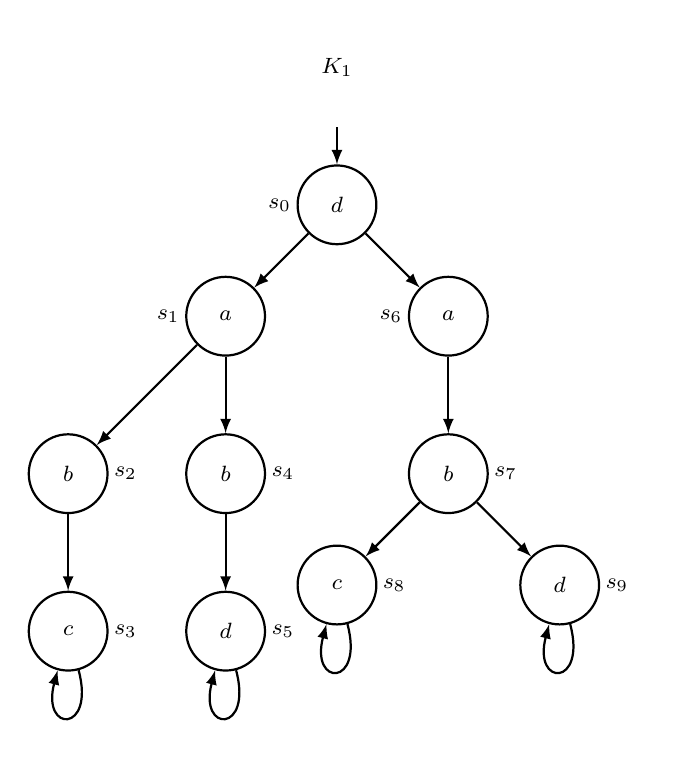
\begin{tikzpicture}[->,scale=1,label distance=-3mm,>= latex, node distance = 2cm]
    \tikzstyle{every node}=[shape=circle,minimum size=10mm,font=\footnotesize];
    \tikzstyle{every path} = [draw,thick];
    
    \node[draw] (n0) [label=left:$s_0$] {$d$};
    
    \node (tmp) [above of=n0, node distance=1.5cm] {};
    \node (tmp2) [above of=tmp,node distance=0.25cm] {$K_1$};
    
    \node[draw] (n6) [below right of=n0,label=left:$s_6$] {$a$};
    \node[draw] (n1) [below left of=n0,label=left:$s_1$] {$a$};
    \node[draw] (n4) [below of=n1,label=right:$s_4$] {$b$};
    \node[draw] (n2) [left of=n4,label=right:$s_2$] {$b$};
    \node[draw] (n3) [below of=n2,label=right:$s_3$] {$c$};
    \node[draw] (n5) [below of=n4,label=right:$s_5$] {$d$};
    \node[draw] (n8) [below of=n6,label=right:$s_7$] {$b$};
    \node[draw] (n9) [below left of=n8,label=right:$s_8$] {$c$};
    \node[draw] (n10) [below right of=n8,label=right:$s_{9}$] {$d$};
    
    \draw[->] (tmp) -- (n0);
    \draw[->] (n0) -- (n1);
    \draw[->] (n0) -- (n6);
    \draw[->] (n1) -- (n2);
    \draw[->] (n1) -- (n4);
    \draw[->] (n2) -- (n3);
    \draw[->] (n4) -- (n5);
		\draw[->] (n6) -- (n8);
		\draw[->] (n8) -- (n9);
		\draw[->] (n8) -- (n10);
		    
    \path[loop below] (n3) to (n3);
    \path[loop below] (n5) to (n5);
    \path[loop below] (n9) to (n9);
    \path[loop below] (n10) to (n10);
    
\end{tikzpicture}
}
\end{minipage}
\hfill
\begin{minipage}{0.48\textwidth}
	\scalebox{0.8}{
  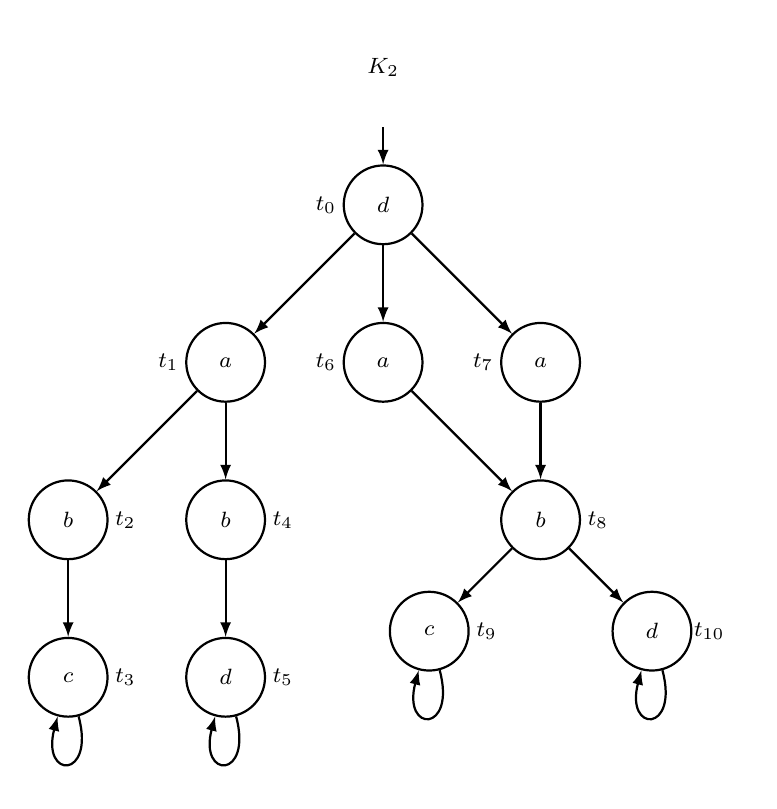
\begin{tikzpicture}[->,scale=1,label distance=-3mm,>= latex, node distance = 2cm]
    \tikzstyle{every node}=[shape=circle,minimum size=10mm,font=\footnotesize];
    \tikzstyle{every path} = [draw,thick];
    
    \node[draw] (n0) [label=left:$t_0$] {$d$};
    
    \node (tmp) [above of=n0, node distance=1.5cm] {};
    \node (tmp2) [above of=tmp,node distance=0.25cm] {$K_2$};
    
    \node[draw] (n6) [below of=n0,label=left:$t_6$] {$a$};
    \node[draw] (n1) [left of=n6,label=left:$t_1$] {$a$};
    \node[draw] (n7) [right of=n6,label=left:$t_7$] {$a$};
    \node[draw] (n4) [below of=n1,label=right:$t_4$] {$b$};
    \node[draw] (n2) [left of=n4,label=right:$t_2$] {$b$};
    \node[draw] (n3) [below of=n2,label=right:$t_3$] {$c$};
    \node[draw] (n5) [below of=n4,label=right:$t_5$] {$d$};
    \node[draw] (n8) [below of=n7,label=right:$t_8$] {$b$};
    \node[draw] (n9) [below left of=n8,label=right:$t_9$] {$c$};
    \node[draw] (n10) [below right of=n8,label=right:$t_{10}$] {$d$};
    
    \draw[->] (tmp) -- (n0);
    \draw[->] (n0) -- (n1);
    \draw[->] (n0) -- (n6);
    \draw[->] (n0) -- (n7);
    \draw[->] (n1) -- (n2);
    \draw[->] (n1) -- (n4);
    \draw[->] (n2) -- (n3);
    \draw[->] (n4) -- (n5);
		\draw[->] (n6) -- (n8);
		\draw[->] (n7) -- (n8);
		\draw[->] (n8) -- (n9);
		\draw[->] (n8) -- (n10);
		    
    \path[loop below] (n3) to (n3);
    \path[loop below] (n5) to (n5);
    \path[loop below] (n9) to (n9);
    \path[loop below] (n10) to (n10);
    
\end{tikzpicture}
}
\end{minipage}
\end{center}


\paragraph{a)} Give a simulation relation $H'$ such that $K_1 \leq K_2$ and $|H'| < |H|$.\hfill\textbf{(0.5 Points)}

\paragraph{b)} Give a simulation relation $H''$ such that $K_1 \leq K_2$ and $|H''| > |H|$.\hfill\textbf{(0.5 Points)}

\newpage
\Aufgabe[Simulation as refinement \hfill\textbf{(2 Points)}]
 
Given a \texttt{C} program and a set $AP$ of atomic propositions,
one can construct a Kripke structure over $AP$ which models the behaviour of the program with respect to the atomic propositions. 
For example, given the following program:

\begin{verbatim}
int x = 0, y = 0;
l0:
    y = 0;
    for (int i = 0; i < 2; i++)
l1:     x = 1;
    y = *;
    if (y != 0)
l2:     x = 1;
    else
l3:     x = 0;
    goto l0;
\end{verbatim}

One may construct the following Kripke structure over $AP=\{x=0, y=0\}$
as follows:

\begin{center}
	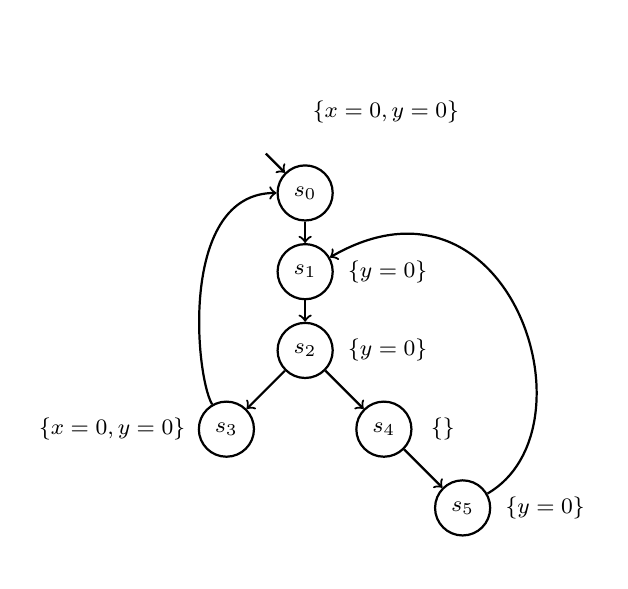
\begin{tikzpicture}[->,scale=1,label distance=0mm]
		\tikzstyle{every node}=[draw,shape=circle,minimum size=7mm,font=\footnotesize];
    \tikzstyle{every path}=[draw,thick];
    \node at (0, 0)   (s0) [label=above right:${ \{x=0,y=0\} }$]  {$s_0$};
    \node at (0, -1)  (s1) [label=right:${ \{y=0\} }$] {$s_1$};
    \node at (0, -2)  (s2) [label=right:${ \{y=0\} }$] {$s_2$};
    \node at (-1, -3) (s3) [label=left:${ \{x=0,y=0\} }$] {$s_3$};
    \node at (1, -3)  (s4) [label=right:${\{ \} }$] {$s_4$};
    \node at (2, -4)  (s5) [label=right:${\{ y = 0 \} }$] {$s_5$};

    \draw (-0.5, 0.5) to (s0);
    \draw (s0) to (s1);
    \draw (s1) to (s2);
    \draw (s2) to (s3);
    \draw (s2) to (s4);
    \draw (s3) .. controls +(120:8mm) and +(left:16mm) .. (s0);
    \draw (s4) to (s5);
    \draw (s5) .. controls +(30:20mm) and +(30:30mm) .. (s1);
	\end{tikzpicture}
\end{center}
In the example above, the special
form of assignment \texttt{y = *} denotes a non-deterministic assignment
to~\texttt{y} of any value from the domain of \texttt{y}, e.g., it can be
assigned concurrently by another thread.
The effect of a statement sequence residing under the same label $\ell_j$ may
be merged into one state, whereas the effect of statements marked with
distinct labels $\ell_j$ and $\ell_k$, $j \ne k$, must not be merged into one
state.

\paragraph{a)}
Construct a Kripke structure $K$ over
$AP=\{port\_o=0,port\_o=1,port\_o=2,port\_o=3\}$ for the following program:

\begin{verbatim}
int locked_dev = 0, port_o = 0, port_i = 0;
l0:
    for (int i = 0; i < 3; i++)
l1:     port_o = 1;

    port_i = *;
    if (port_i < 3) {
        goto l0;
    }
    do {
l2:     port_o = 2; locked_dev = *;
    } while (locked_dev);
l3: locked_dev = 1; port_i = *;
    if (port_i == 1)
l4:     port_o = 1;
    else
l5:     port_o = 3;
l6: port_o = 0; locked_dev = 0;
    goto l0;
\end{verbatim}


\paragraph{b)}
Give simulation relations between $K$ and the following Kripke structures
 $S'$ (left) and $S''$ (right):

\begin{center}
	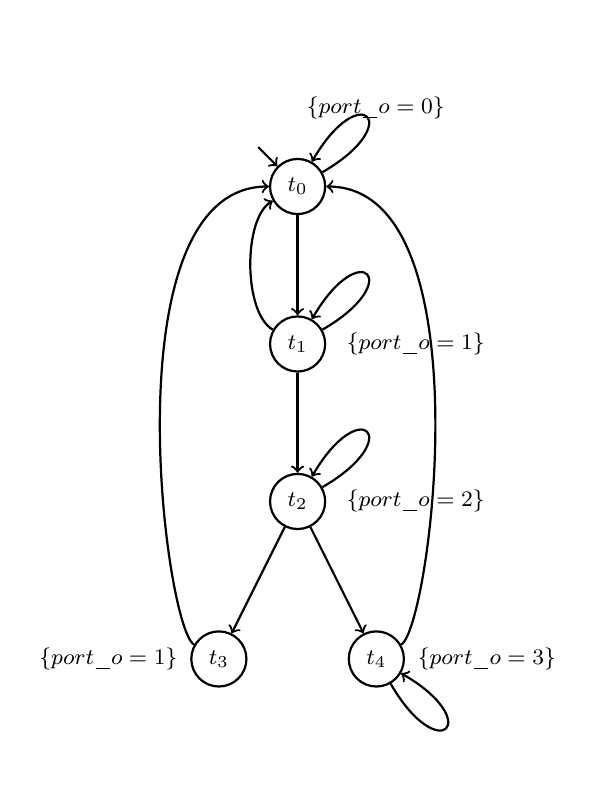
\begin{tikzpicture}[->,scale=1,label distance=0mm]
		\tikzstyle{every node}=[draw,shape=circle,minimum size=7mm,font=\footnotesize];
    \tikzstyle{every path}=[draw,thick];
    \node at (0, 0)   (s0) [label=above right:${ \{port\_o=0\} }$]  {$t_0$};
    \node at (0, -2)  (s1) [label=right:${ \ \{port\_o=1\} }$] {$t_1$};
    \node at (0, -4)  (s2) [label=right:${ \ \{port\_o=2\} }$] {$t_2$};
    \node at (-1, -6) (s3) [label=left:${ \{port\_o=1\} }$] {$t_3$};
    \node at (1, -6)  (s4) [label=right:${ \{port\_o=3\} }$] {$t_4$};

    \draw (-0.5, 0.5) to (s0);
    \draw (s0) to (s1);
    \draw (s0)  .. controls +(30:16mm) and +(60:16mm) .. (s0);
    \draw (s1)  .. controls +(150:8mm) and +(210:8mm) .. (s0);
    \draw (s1)  .. controls +(30:16mm) and +(60:16mm) .. (s1);
    \draw (s1) to (s2);
    \draw (s2)  .. controls +(30:16mm) and +(60:16mm) .. (s2);
    \draw (s2) to (s3);
    \draw (s2) to (s4);
    \draw (s3) .. controls +(150:8mm) and +(left:24mm) .. (s0);
    \draw (s4) .. controls +(30:8mm) and +(right:24mm) .. (s0);
    \draw (s4)  .. controls +(300:16mm) and +(330:16mm) .. (s4);
    	\end{tikzpicture}
	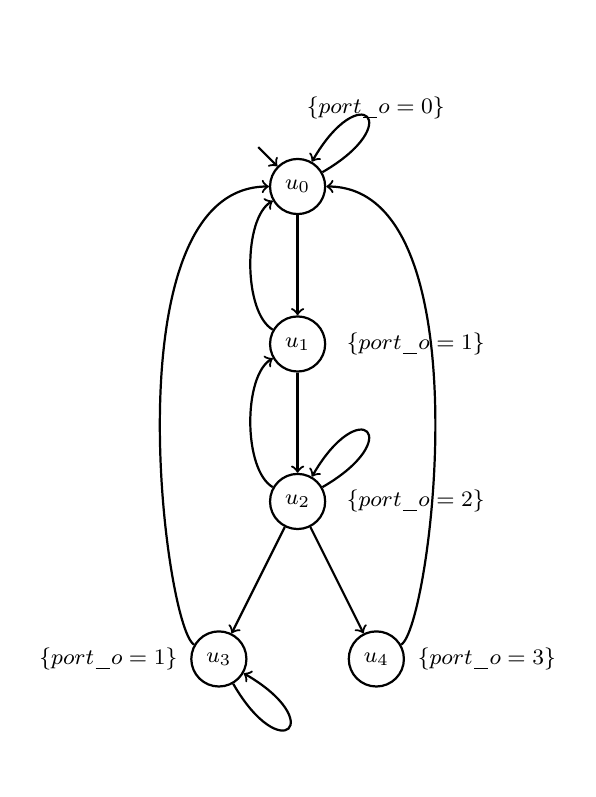
\begin{tikzpicture}[->,scale=1,label distance=0mm]
		\tikzstyle{every node}=[draw,shape=circle,minimum size=7mm,font=\footnotesize];
    \tikzstyle{every path}=[draw,thick];
    \node at (0, 0)   (s0) [label=above right:${ \{port\_o=0\} }$]  {$u_0$};
    \node at (0, -2)  (s1) [label=right:${ \ \{port\_o=1\} }$] {$u_1$};
    \node at (0, -4)  (s2) [label=right:${ \ \{port\_o=2\} }$] {$u_2$};
    \node at (-1, -6) (s3) [label=left:${ \{port\_o=1\} }$] {$u_3$};
    \node at (1, -6)  (s4) [label=right:${ \{port\_o=3\} }$] {$u_4$};

    \draw (-0.5, 0.5) to (s0);
    \draw (s0) to (s1);
    \draw (s0)  .. controls +(30:16mm) and +(60:16mm) .. (s0);
    \draw (s1)  .. controls +(150:8mm) and +(210:8mm) .. (s0);
    \draw (s2)  .. controls +(150:8mm) and +(210:8mm) .. (s1);
    \draw (s1) to (s2);
    \draw (s2)  .. controls +(30:16mm) and +(60:16mm) .. (s2);
    \draw (s2) to (s3);
    \draw (s2) to (s4);
    \draw (s3) .. controls +(150:8mm) and +(left:24mm) .. (s0);
    \draw (s3) .. controls +(300:16mm) and +(330:16mm) .. (s3);
    \draw (s4) .. controls +(30:8mm) and +(right:24mm) .. (s0);
    	\end{tikzpicture}
\end{center}

\newpage
\Aufgabe[Predicate Abstraction\hfill\textbf{(1.5 Point)}]
Consider the following program:
\begin{verbatim}
void foo(int j, int z) {
  assume(z != 0);
  int i := j;
  while(z != 0) {
      i := i + z;
      if(z > 0)
          z--
      else
          z ++;
  };
  assert(i != j)
}
\end{verbatim}

The {\em assume statement} at the beginning of the function forces the parameter $z$ not to be 0 when the function is called.

\begin{enumerate}

 \item Argue in your own words why the assertion at the end of the program allways holds, i.e., why the error state can never be reached.

Because of the precondition $assume(z\neq0)$, the while-loop is executed at least one time, no matter of the sign of $z$.
Because of the $if$ - statement inside the loop, the loop is executed exactely $|z|$ - times, with every execution of the loop incrementing or decrementing the variable $i$,
while $j$ is not changed in the program. But because $i=j$ before the loop and the guaranteed execution of loop, $i=j$ cannot hold after the loop.
 \item Provide a labeled transition system for the given program.

\begin{center}
	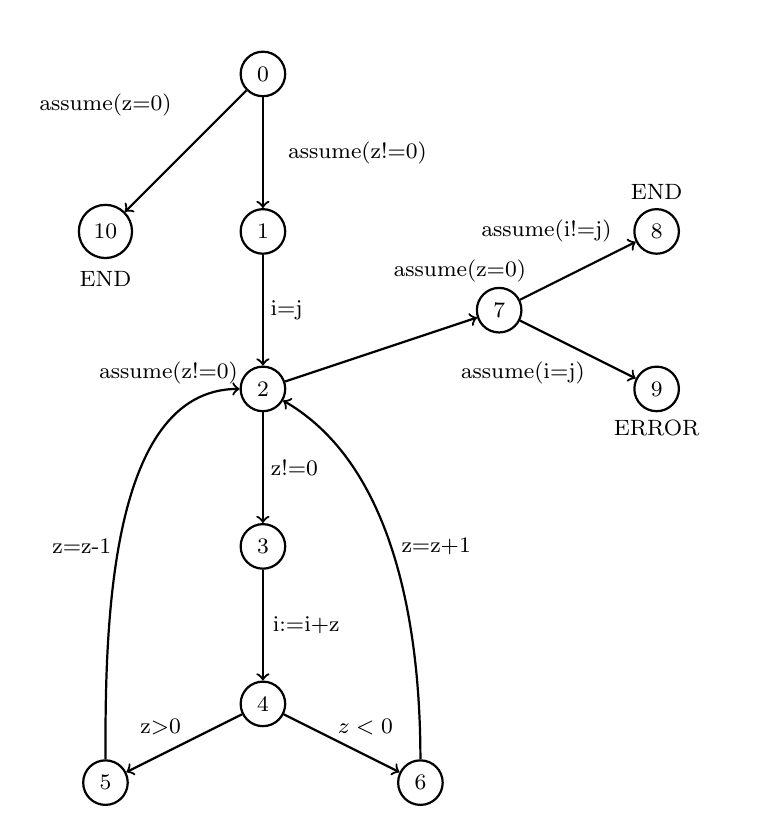
\begin{tikzpicture}[->,scale=1,label distance=0mm,auto]
		\tikzstyle{every node}=[draw,shape=circle,minimum size=5mm,font=\footnotesize];
    \tikzstyle{every path}=[draw,thick];
    \node at (0, 1)   (s0) {$0$};
    \node at (0, -1)  (s1) {$1$};
    \node at (0, -3)  (s2) {$2$};
    \node at (0, -5) (s3) {$3$};
    \node at (0, -7)  (s4) {$4$};
    \node at (-2, -8)  (s5) {$5$};
    \node at (2, -8)  (s6) {$6$};
    \node at (3, -2)  (s7) {$7$};
    \node at (5, -1)  (s8) {$8$};
    \node at (5, -3)  (s9) {$9$};
    \node at (-2, -1)  (s10) {$10$};


\node[draw=none] at (1.2,0) {assume(z!=0)};
\node[draw=none] at (-2,0.6) {assume(z=0)};
\node[draw=none] at (0.3,-2) {i=j};
\node[draw=none] at (0.4,-4) {z!=0};
\node[draw=none] at (0.55,-6) {i:=i+z};
\node[draw=none] at (-1.3,-7.3) {z$>$0};
\node[draw=none] at (1.3,-7.3) {$z<0$};
\node[draw=none] at (-2.3,-5) {z=z-1};
\node[draw=none] at (2.2,-5) {z=z+1};
\node[draw=none,label=right:{}] at (-1.2,-2.8) {assume(z!=0)};
\node[draw=none,label=right:{}] at (2.5,-1.5) {assume(z=0)};

\node[draw=none,label=right:{}] at (-2,-1.6) {END};
\node[draw=none,label=right:{}] at (5,-0.5) {END};
\node[draw=none,label=right:{}] at (5,-3.5) {ERROR};
\node[draw=none,label=right:{}] at (3.6,-1) {assume(i!=j)};
\node[draw=none,label=right:{}] at (3.3,-2.8) {assume(i=j)};


    \draw (s0) to (s10);
    \draw (s0) to (s1);
    \draw (s1) to (s2);
    \draw (s2) to (s3);
    \draw (s2) to (s7);
    \draw (s3) to (s4) ;
    \draw (s4) to (s6) ;
    \draw (s6) .. controls +(up:18mm) and +(330:20mm) .. (s2);
    \draw (s7) to (s8);
    \draw (s7) to (s9);

    \draw (s5) .. controls +(up:18mm) and +(180:20mm) .. (s2);
    \draw (s4) to (s5);
	\end{tikzpicture}
\end{center}



 \item Provide an abstraction for the labeled transition system that uses the predicates $i = j$, $i < j$, $i > j$.

\begin{center}
	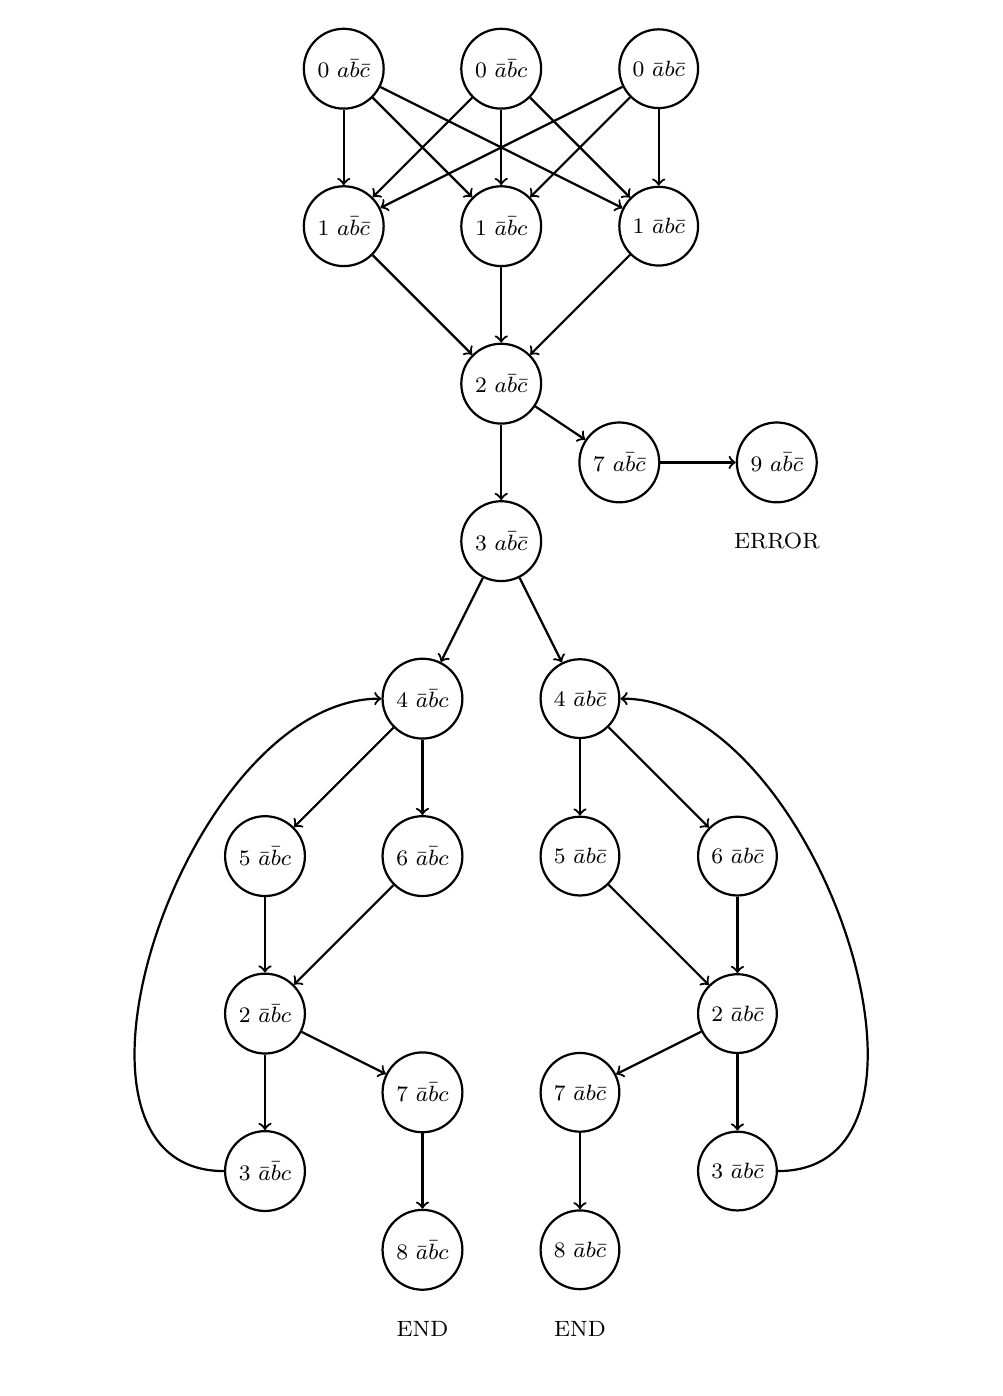
\begin{tikzpicture}[->,scale=1,label distance=0mm,auto]
		\tikzstyle{every node}=[draw,shape=circle,minimum size=10mm,font=\footnotesize];
    \tikzstyle{every path}=[draw,thick];
    \node at (-2, 1)   (sa0) {$0\ a \bar b\bar c$};
    \node at (0, 1)  (sb0) {$0\ \bar a \bar b c$};
    \node at (2, 1)  (sc0) {$0\ \bar a b \bar c$};
	\node at (-2, -1)   (sa1) {$1\ a \bar b\bar c$};
    \node at (0, -1)  (sb1) {$1\ \bar a \bar b c$};
    \node at (2, -1)  (sc1) {$1\ \bar a b\bar c$};
    \node at (0, -3)  (s2) {$2\ a \bar b\bar c$};
    \node at (0, -5)  (s3) {$3\ a \bar b\bar c$};
    \node at (-1, -7)  (s4a) {$4\ \bar a \bar b c$};
    \node at (1, -7)  (s4b) {$4\ \bar a b \bar c$};
	\node at (-3, -9)  (s5a) {$5\ \bar a \bar b c$};
    \node at (-1, -9)  (s6a) {$6\ \bar a \bar b c$};
    \node at (1, -9)  (s5b) {$5\ \bar a b \bar c$};
    \node at (3, -9)  (s6b) {$6\ \bar a b \bar c$};
\node at (-3, -11)  (s2a) {$2\ \bar a \bar b c$};
    \node at (3, -11)  (s2b) {$2\ \bar a b \bar c$};
\node at (-3, -13)  (s3a) {$3\ \bar a \bar b c$};
    \node at (3, -13)  (s3b) {$3\ \bar a b \bar c$};
    \node at (-1, -12)  (s7a) {$7\ \bar a \bar b c$};
    \node at (1, -12)  (s7b) {$7\ \bar a b \bar c$};
  \node at (-1, -14)  (s8a) {$8\ \bar a \bar b c$};
    \node at (1, -14)  (s8b) {$8\ \bar a b \bar c$};
 \node at (1.5, -4)  (s7c) {$7\ a \bar b\bar c$};
    \node at (3.5, -4)  (s9) {$9\ a \bar b\bar c$};
\node[draw=none,label=right:{}] at (3.5,-5) {ERROR};
\draw (s2) to (s7c);
\draw (s7c) to (s9);
\draw (sa0) to (sa1);
\draw (sa0) to (sb1);
\draw (sa0) to (sc1);
\draw (sb0) to (sa1);
\draw (sb0) to (sb1);
\draw (sb0) to (sc1);
\draw (sc0) to (sa1);
\draw (sc0) to (sb1);
\draw (sc0) to (sc1);
\draw (sa1) to (s2);
\draw (sb1) to (s2);
\draw (sc1) to (s2);
\draw (s2) to (s3);
\draw (s3) to (s4a);
\draw (s3) to (s4b);
\draw (s4a) to (s5a);
\draw (s4a) to (s6a);
\draw (s4b) to (s5b);
\draw (s4b) to (s6b);
\draw (s5a) to (s2a);
\draw (s6a) to (s2a);
\draw (s5b) to (s2b);
\draw (s6b) to (s2b);
\draw (s2a) to (s3a);
\draw (s2b) to (s3b);
\draw (s2a) to (s7a);
\draw (s2b) to (s7b);
\draw (s7a) to (s8a);
\draw (s7b) to (s8b);

\draw (s3a) .. controls +(left:30mm) and +(left:30mm) .. (s4a);
\draw (s3b) .. controls +(right:30mm) and +(right:30mm) .. (s4b);

\node[draw=none,label=right:{}] at (-1,-15) {END};
\node[draw=none,label=right:{}] at (1,-15) {END};


	\end{tikzpicture}
\end{center}

 \item Check whether the error state can be reached in the abstraction, if so state a trace to the error state and refine the abstraction with suitable predicates such that the error state is not reachable anymore.

 The error state can  be reached in the abstraction since we don´t have information about z. If we update the abstraction with a predicate for (z != 0) we can be sure that we can´t reach the error state again. 

\begin{center}
	\begin{tikzpicture}[->,scale=1,label distance=0mm,auto]
		\tikzstyle{every node}=[draw,shape=circle,minimum size=10mm,font=\footnotesize];
    \tikzstyle{every path}=[draw,thick];
    \node at (-2, 1)   (sa0) {$0\ a \bar b\bar c$};

    \node at (2, -1)  (sc1) {$1\ \bar a b\bar c$};
    \node at (0, -3)  (s2) {$2\ a \bar b\bar c$};   
    \node at (1.5, -4)  (s7c) {$7\ a \bar b\bar c$};
    \node at (3.5, -4)  (s9) {$9\ a \bar b\bar c$};
\node[draw=none,label=right:{}] at (3.5,-5) {ERROR};

\draw (s2) to (s7c);
\draw (s7c) to (s9);
\draw (sa0) to (sc1);
\draw (sc1) to (s2);
\draw (s2) to (s3);

\end{tikzpicture}
\end{center}



\end{enumerate}

\newpage
%%%%%%%%%%%%%%%%%%%%%%%%%%%%%%%%%%%%%%%%%%%%%%%%%%%%%%%%%%%%%%%%%%%%%%
%% Aufgabe
\Aufgabe[Bounded Model Checking\hfill\textbf{(1.5 Point)}]
Consider the following Program:

\lstinputlisting[basicstyle=\footnotesize]{main.c}

The Matrix $G$ models a graph with $N$ nodes, i.e, $G[i][j]$ is true iff there is a directed edge from node $i$ to node $j$. The method $\mathit{nondet}$ chooses an integer non-deterministically.

\begin{enumerate}
	\item Use CBMC to find the lowest value for $K$ such that the assertion at the end of the program can be violated. What does it mean that the error state is or is not reachable for a given graph $G$ and a given value $K$?
	  
	$K=2$ is the smallest number for which the assertion is violated. Because the assertion is reversed this means that there is always a path with length=1.

	\item Perform an unwinding of the loop for $K = 3$.
	\item Transform the unwinded program into the SSA form.
	\item Build an SMT formula from the SSA form which is satisfiable if and only if the assertion at the end of the program may be violated. {\em Note:} A call to $\mathit{nondet}$ can be modeled by introducing a new integer variable.
        \item Can you draw a conclusion about the satisfiability of the formula by comparing the value for $K$ that you determined under $(a)$ with the number of times the loop was unwinded for building the formula? Check whether the formula can be satisfied (You may use an SMT solver such as {\em Yices} or {\em Z3}) to be sure that the result of the satisfiability check is consistent with your expectation.
\end{enumerate}


\newpage
\Aufgabe[Computing the (Greatest) Bisimulation Relation \hfill\textbf{(1 Point)}]

Let $K_1 = (S_1, R_1, L_1)$ and  $K_2 = (S_2, R_2, L_2)$ be two Kripke structures over a set of atomic predicates $\mathit{AP}$.
The relations $H_n \subseteq S_1 \times S_2$ are inductively defined by:
\begin{itemize}
\item $(s_1,s_2) \in H_0$ iff $L_1(s_1) = L_2(s_2)$.
\item $(s_1,s_2) \in H_{n+1}$ iff
    \begin{enumerate}[(i)]
    \item $(s_1,s_2) \in H_n$,
    \item for all $(s_1,t_1) \in R_1$ there exists a $(s_2,t_2) \in R_2$ with $(t_1,t_2) \in H_n$, and
    \item for all $(s_2,t_2) \in R_2$ there exists a $(s_1,t_1) \in R_1$ with $(t_1,t_2) \in H_n$.
    \end{enumerate}
\end{itemize}

\begin{enumerate}

	\item Compute the sequence $H_0, H_1, H_2,\ldots$ for the Kripke structures $K_1$ and $K_2$ from Exercise 2.
    
	\item Show that the sequence $H_0, H_1, H_2,\ldots$ \emph{stabilizes} for all finite Kripke structures $K_1$ and $K_2$, i.e., there is a $n \ge 0$ such that $H_n = H_{n+1}$.
    
	\item Construct Kripke structures $K_1^n$ and $K_2^n$ such that the sequence $H_0, H_1, H_2,\ldots$ stabilizes after exactly $n$ steps.

\end{enumerate}

\newpage
%\input{ltl_fo}
%\newpage



\end{document}

